% Preliminary results for the PQK100 project.
% Tables, figures, and every number quoted below are generated by notebook 5
% (05_tables_and_figures.ipynb) from the files in results/. Do not edit tables/ by hand.
%
% Compile:  pdflatex pqk100_preliminary  (twice)
\documentclass[aps,pra,reprint,superscriptaddress,nofootinbib,floatfix]{revtex4-2}
\usepackage{amsmath,amssymb,bm}
\usepackage{graphicx}
\usepackage{booktabs}
\usepackage{placeins}
\usepackage[colorlinks=true,allcolors=blue]{hyperref}

% Generated by notebook 5. Do not edit by hand.
\newcommand{\NTcga}{1,082}
\newcommand{\NMeta}{1,980}
\newcommand{\NGenes}{17,139}
\newcommand{\NSeeds}{5}
\newcommand{\Lattice}{ibm\_fez}
\newcommand{\MaxAbsDiff}{0.017}
\newcommand{\SeMin}{0.001}
\newcommand{\SeMax}{0.021}
\newcommand{\SelSmall}{28}
\newcommand{\SelMid}{7}
\newcommand{\SelLarge}{0}
\newcommand{\SelTotal}{35}
\newcommand{\RefIn}{0.918}
\newcommand{\RefExt}{0.890}
\newcommand{\BlochSmallMin}{0.98}
\newcommand{\BlochSmallMax}{0.99}
\newcommand{\BlochLargeMin}{0.69}
\newcommand{\BlochLargeMax}{0.75}
\newcommand{\LossLargeMin}{0.03}
\newcommand{\LossLargeMax}{0.06}
\newcommand{\ConcBloch}{0.06}
\newcommand{\ConcSpread}{0.02}
\newcommand{\GeoMeanMin}{1.1}
\newcommand{\GeoMeanMax}{1.9}
\newcommand{\GeoMax}{8.2}
\newcommand{\EpsCZ}{0.0039}
\newcommand{\ProxyEps}{0.0039}
\newcommand{\ShotUs}{253}
\newcommand{\RepDelayUs}{250}
\newcommand{\CircuitUs}{1.5}
\newcommand{\MinFull}{12}
\newcommand{\MinFullHigh}{47}
\newcommand{\MinPilot}{1.6}
\newcommand{\MpsEight}{3.1\times10^{-2}}
\newcommand{\MpsThirtyTwo}{4.5\times10^{-4}}
\newcommand{\MpsSixtyFour}{1.9\times10^{-5}}

\newcommand{\ev}[1]{\langle #1 \rangle}

\begin{document}

\title{Projected quantum kernels on up to 156 qubits for genomic classification\\ with an independent validation cohort: preliminary results}

\author{Muhammad Faryad}
\affiliation{Department of Physics, Syed Babar Ali School of Science and Engineering,\\ Lahore University of Management Sciences, Lahore 54792, Pakistan}

\date{\today}

\begin{abstract}
Working draft. This file holds the setup and the preliminary numerical results only.
All results are exact noiseless simulations on the heavy-hex lattice of \Lattice. No hardware data are included yet.
The introduction, the hardware results, and the discussion are still to be written.
\end{abstract}

\maketitle

% ---------------------------------------------------------------------------
% \section{Introduction}
% TO WRITE. Prior work to position against: 61-qubit PQK on CAR T-cell data (arXiv:2507.22710),
% 100-qubit PQK Gaussian process for time series (arXiv:2605.24252),
% 156-qubit fidelity kernels with bit-flip tolerance (arXiv:2412.07915).
% ---------------------------------------------------------------------------

\section{Setup}

\subsection{Cohorts and task}

The task is binary: predict the somatic \textit{TP53} mutation status of a primary breast tumor from its gene expression.
The training cohort is TCGA-BRCA~\cite{tcga2012,ciriello2015,hoadley2018}, with RNA-seq expression (RSEM, transformed as $\log_2(x+1)$).
The validation cohort is METABRIC~\cite{curtis2012,pereira2016}, with Illumina microarray expression.
Both were obtained from cBioPortal~\cite{cerami2012,gao2013}.
The two cohorts share \NGenes{} genes.
A tumor is labeled positive if it carries a non-silent somatic \textit{TP53} mutation.
Table~\ref{tab:cohorts} lists the cohort sizes.
The label comes from DNA sequencing and is independent of the expression data.

\begin{table}
\caption{\label{tab:cohorts}Cohorts. Tumors with a \textit{TP53} call are those with both expression and sequencing data.}
\resizebox{\columnwidth}{!}{\begin{tabular}{llrrr}
\toprule
Cohort & Platform & Tumors & \textit{TP53} call & Mutated (\%) \\
\midrule
TCGA-BRCA & RNA-seq (RSEM) & 1,082 & 811 & 34.4 \\
METABRIC & Illumina HT-12 microarray & 1,980 & 1,904 & 34.6 \\
\bottomrule
\end{tabular}
}
\end{table}

Two other tasks were screened with classical models and rejected (Table~\ref{tab:screen}).
Estrogen receptor status is solved by \textit{ESR1} alone.
The PAM50 luminal A versus B label is itself computed from expression and leaves little headroom.

\begin{table}
\caption{\label{tab:screen}Task screen with logistic regression. ROC AUC on held-out TCGA-BRCA and on METABRIC, 200 training tumors, mean of 3 resamples.}
\resizebox{\columnwidth}{!}{\begin{tabular}{llcccc}
\toprule
 & & \multicolumn{2}{c}{Best single gene} & \multicolumn{2}{c}{156 genes} \\
\cmidrule(lr){3-4}\cmidrule(lr){5-6}
Task & Top gene & TCGA & METABRIC & TCGA & METABRIC \\
\midrule
ER status (IHC) & \textit{ESR1} & 0.957 & 0.957 & 0.951 & 0.941 \\
Luminal A vs B (PAM50) & \textit{SPAG5} & 0.882 & 0.840 & 0.973 & 0.929 \\
TP53 mutation & \textit{TBC1D9} & 0.864 & 0.791 & 0.925 & 0.874 \\
\bottomrule
\end{tabular}
}
\end{table}

\subsection{Preprocessing and gene selection}

Each gene is standardized within its own cohort. This uses no labels, but it does use the unlabeled validation data.
A per-sample rank normalization, which uses no cohort statistics, is reported as a control in Sec.~\ref{sec:ablation}.
The 5{,}000 most variable genes of the training subset are kept.
Genes are then ranked on the training subset by the ANOVA $F$ statistic, skipping any gene whose absolute correlation with an already selected gene exceeds $0.8$.
The first $n$ genes form the panel for an $n$-qubit circuit, so panels are nested.
No label from the held-out or validation tumors enters any of these steps.

\subsection{Feature map and lattice}

One gene is assigned to each qubit. The rotation angle of gene $j$ is
\begin{equation}
x_j = \beta\,\mathrm{clip}(z_j,-3,3),
\end{equation}
where $z_j$ is the standardized expression and $\beta$ is the bandwidth in radians per standard deviation.
The feature map repeats one block $R$ times,
\begin{equation}
U(\mathbf{x}) = \Bigl[\,\prod_{(j,k)\in E} e^{-\frac{i}{2} x_j x_k Z_j Z_k}\;\prod_{j} e^{-\frac{i}{2} x_j Z_j}\; H^{\otimes n}\Bigr]^{R},
\label{eq:map}
\end{equation}
acting on $|0\rangle^{\otimes n}$. Here $E$ is the set of couplers of an $n$-qubit patch of the 156-qubit heavy-hex lattice of \Lattice.
The patch is built by removing qubits one at a time, worst first by readout error plus mean two-qubit error, never disconnecting the patch.
All two-qubit gates act on native couplers, so no routing is needed.
The couplers split into three layers of disjoint gates. In the CZ basis one repetition has CZ depth 6.

\subsection{Projected quantum kernel}

For each tumor we take the single-qubit expectation values $\ev{P_k}_{\mathbf{x}}$, $P\in\{X,Y,Z\}$, $k=1,\dots,n$, in the state $U(\mathbf{x})|0\rangle^{\otimes n}$.
The projected quantum kernel (PQK)~\cite{huang2021} is
\begin{equation}
k(\mathbf{x},\mathbf{x}') = \exp\Bigl[-\gamma \sum_{k=1}^{n}\sum_{P\in\{X,Y,Z\}} \bigl(\ev{P_k}_{\mathbf{x}}-\ev{P_k}_{\mathbf{x}'}\bigr)^2\Bigr].
\label{eq:pqk}
\end{equation}
It needs three measurement settings per tumor, independent of the number of training samples.
A support vector machine is trained on this kernel.

\subsection{Baselines and protocol}

The classical baselines are an RBF-kernel support vector machine (RBF-SVM), $\ell_2$-regularized logistic regression (LogReg), and gradient-boosted trees (GBM), all from scikit-learn~\cite{sklearn}.
They receive the same $n$ standardized genes as the circuit.
The PQK and the RBF-SVM are tuned on the same grid of $C$ and $\gamma$. All tuning uses 5-fold cross-validation on the training subset with ROC AUC as the score.
The depth $R\in\{1,2,3\}$ and the bandwidth $\beta\in\{0.25,0.5,1\}$ of the feature map are chosen the same way.

Each resample draws 200 training tumors from TCGA-BRCA, 200 further TCGA-BRCA tumors as the held-out set, and 400 METABRIC tumors as the independent set, all stratified by class.
Results are means over \NSeeds{} resamples. The resamples share the same two cohorts, so the quoted standard errors are optimistic.

\subsection{Exact simulation}
\label{sec:sim}

The expectation value $\ev{P_k}$ depends only on the gates in the backward light cone of qubit $k$.
The $ZZ$ rotations of one repetition commute, so the cone grows by one lattice step per repetition.
Table~\ref{tab:cones} gives the cone sizes on the full 156-qubit lattice.
For $R\le 4$ every single-qubit reduced density matrix is a statevector calculation on at most 19 qubits.
All results below use this method and are exact up to floating-point error.

\begin{table}
\caption{\label{tab:cones}Light cones of the map in Eq.~(\ref{eq:map}) on all 156 qubits of \Lattice. Cone sizes are in qubits.}
\resizebox{\columnwidth}{!}{\begin{tabular}{cccccc}
\toprule
$R$ & Largest cone & Mean cone & CZ in largest cone & CZ in circuit & CZ depth \\
\midrule
1 & 4 & 3.3 & 6 & 352 & 6 \\
2 & 7 & 6.4 & 18 & 704 & 12 \\
3 & 13 & 10.3 & 42 & 1,056 & 18 \\
4 & 19 & 15.8 & 78 & 1,408 & 24 \\
5 & 31 & 22.7 & 138 & 1,760 & 30 \\
6 & 41 & 30.7 & 222 & 2,112 & 36 \\
\bottomrule
\end{tabular}
}
\end{table}

The simulator was checked in two ways.
On 16-qubit patches it agrees with a full statevector simulation in Qiskit~\cite{qiskit} to within $2\times10^{-13}$.
On the full 156-qubit circuit at $R=2$, a matrix-product-state simulation converges to the same values:
the largest deviation is $\MpsEight$, $\MpsThirtyTwo$, and $\MpsSixtyFour$ at bond dimension 8, 32, and 64.

% ---------------------------------------------------------------------------
\section{Preliminary results}

\subsection{Scaling from 20 to 156 qubits}

Figure~\ref{fig:scaling} and Table~\ref{tab:main} compare the PQK with the classical baselines as the panel grows from 20 to 156 genes.
The PQK tracks the RBF-SVM and logistic regression on both cohorts.
The paired differences in Table~\ref{tab:paired} stay within \MaxAbsDiff{} in AUC and change sign from size to size; their standard errors range from \SeMin{} to \SeMax.
Logistic regression on all 5{,}000 prefiltered genes reaches \RefIn{} on held-out TCGA-BRCA and \RefExt{} on METABRIC.

\begin{figure*}
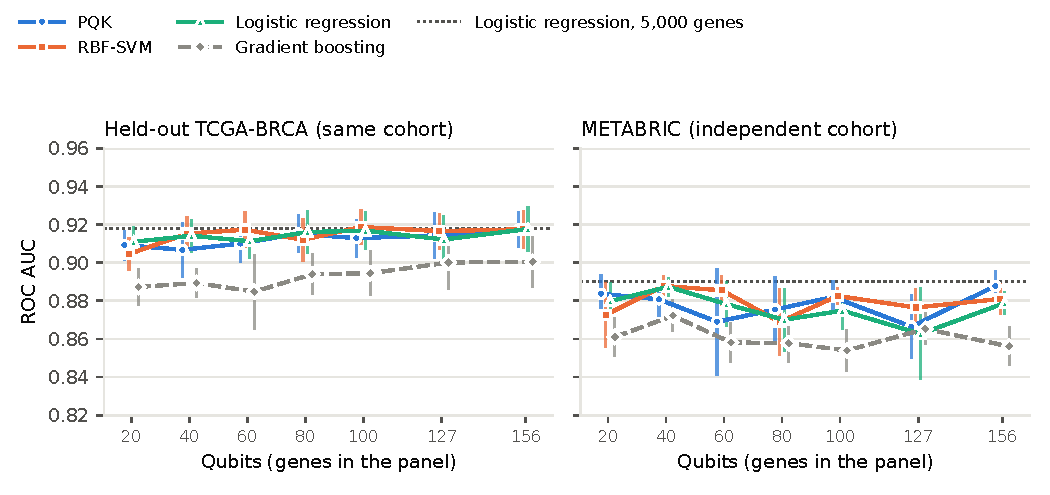
\includegraphics[width=0.9\textwidth]{figures/scaling_auc.pdf}
\caption{\label{fig:scaling}ROC AUC against the number of qubits, which equals the number of genes in the panel.
Left: held-out TCGA-BRCA tumors. Right: the independent METABRIC cohort.
The PQK is computed by exact noiseless simulation, with depth and bandwidth chosen by cross-validation on the training set.
Points are means over \NSeeds{} resamples and bars are one standard error. Points are offset horizontally for clarity.}
\end{figure*}

\begin{table*}
\caption{\label{tab:main}ROC AUC, mean over \NSeeds{} resamples. The number in parentheses is the standard error in units of the last digit.}
\begin{tabular}{rcccccccc}
\toprule
 & \multicolumn{4}{c}{Held-out TCGA-BRCA} & \multicolumn{4}{c}{METABRIC} \\
\cmidrule(lr){2-5}\cmidrule(lr){6-9}
Qubits & PQK & RBF-SVM & LogReg & GBM & PQK & RBF-SVM & LogReg & GBM \\
\midrule
20 & 0.909(8) & 0.904(9) & 0.911(8) & 0.887(10) & 0.884(10) & 0.873(17) & 0.880(10) & 0.861(10) \\
40 & 0.907(14) & 0.915(9) & 0.914(9) & 0.889(8) & 0.881(9) & 0.888(5) & 0.887(5) & 0.872(8) \\
60 & 0.910(10) & 0.917(9) & 0.911(9) & 0.885(20) & 0.869(28) & 0.886(8) & 0.878(12) & 0.858(11) \\
80 & 0.915(10) & 0.912(11) & 0.916(11) & 0.894(11) & 0.875(17) & 0.869(17) & 0.870(16) & 0.858(10) \\
100 & 0.913(10) & 0.919(9) & 0.917(10) & 0.894(12) & 0.882(8) & 0.883(4) & 0.875(10) & 0.854(11) \\
127 & 0.914(12) & 0.917(9) & 0.912(12) & 0.900(14) & 0.866(17) & 0.876(10) & 0.863(24) & 0.865(8) \\
156 & 0.917(10) & 0.917(10) & 0.918(12) & 0.900(13) & 0.888(8) & 0.881(8) & 0.879(6) & 0.856(10) \\
\bottomrule
\end{tabular}

\end{table*}

\begin{table}
\caption{\label{tab:paired}Difference in ROC AUC between the PQK and a classical model, paired by resample. Mean $\pm$ standard error.}
\resizebox{\columnwidth}{!}{\begin{tabular}{rcccc}
\toprule
 & \multicolumn{2}{c}{PQK $-$ RBF-SVM} & \multicolumn{2}{c}{PQK $-$ LogReg} \\
\cmidrule(lr){2-3}\cmidrule(lr){4-5}
Qubits & TCGA & METABRIC & TCGA & METABRIC \\
\midrule
20 & $+0.005\pm0.008$ & $+0.011\pm0.008$ & $-0.002\pm0.002$ & $+0.004\pm0.002$ \\
40 & $-0.008\pm0.006$ & $-0.007\pm0.005$ & $-0.007\pm0.007$ & $-0.007\pm0.005$ \\
60 & $-0.007\pm0.007$ & $-0.017\pm0.021$ & $-0.001\pm0.006$ & $-0.009\pm0.018$ \\
80 & $+0.003\pm0.002$ & $+0.006\pm0.002$ & $-0.001\pm0.002$ & $+0.005\pm0.006$ \\
100 & $-0.006\pm0.004$ & $-0.001\pm0.005$ & $-0.004\pm0.003$ & $+0.007\pm0.006$ \\
127 & $-0.002\pm0.004$ & $-0.010\pm0.007$ & $+0.002\pm0.002$ & $+0.004\pm0.009$ \\
156 & $-0.000\pm0.001$ & $+0.007\pm0.002$ & $-0.000\pm0.004$ & $+0.009\pm0.006$ \\
\bottomrule
\end{tabular}
}
\end{table}

\subsection{Depth and bandwidth}

Table~\ref{tab:depth} and Fig.~\ref{fig:bandwidth} show the effect of the feature-map hyperparameters, averaged over sizes.
Cross-validation selects $\beta=0.25$ in \SelSmall{} of \SelTotal{} cases and $\beta=0.5$ in \SelMid. The largest bandwidth, $\beta=1$, is selected \SelLarge{} times.
At $\beta=0.25$ the mean Bloch-vector length of the single-qubit states is \BlochSmallMin{} to \BlochSmallMax, so the qubits are close to a product state.
At $\beta=1$ it falls to \BlochLargeMin{}--\BlochLargeMax{} and the METABRIC AUC is lower by \LossLargeMin{} to \LossLargeMax.
The geometric difference~\cite{huang2021} between the PQK and the tuned RBF kernel, computed with regularization $1/C$, averages \GeoMeanMin{} to \GeoMeanMax{} across configurations and does not exceed \GeoMax{} in any single run.
The scale for a possible prediction advantage is $\sqrt{N}\approx 14$ at $N=200$ training samples.

\begin{table}
\caption{\label{tab:depth}PQK by depth $R$ and bandwidth $\beta$, mean over resamples and sizes.
$\overline{|\mathbf{r}|}$ is the mean Bloch-vector length, ``Spread'' is the mean standard deviation of an expectation value across training samples,
$g$ is the geometric difference to the tuned RBF kernel with regularization $1/C$, and ``Selected'' counts how often cross-validation chose the configuration.}
\resizebox{\columnwidth}{!}{\begin{tabular}{cccccccc}
\toprule
$R$ & $\beta$ & TCGA & METABRIC & $\overline{|\mathbf{r}|}$ & Spread & $g$ & Selected \\
\midrule
1 & 0.25 & 0.916 & 0.882 & 0.994 & 0.095 & 1.12 & 17 \\
1 & 0.5 & 0.912 & 0.878 & 0.927 & 0.191 & 1.21 & 2 \\
1 & 1 & 0.885 & 0.852 & 0.692 & 0.258 & 1.81 & 0 \\
2 & 0.25 & 0.915 & 0.880 & 0.994 & 0.113 & 1.24 & 6 \\
2 & 0.5 & 0.908 & 0.880 & 0.936 & 0.228 & 1.32 & 1 \\
2 & 1 & 0.860 & 0.819 & 0.752 & 0.328 & 1.93 & 0 \\
3 & 0.25 & 0.915 & 0.881 & 0.981 & 0.207 & 1.23 & 5 \\
3 & 0.5 & 0.902 & 0.870 & 0.883 & 0.320 & 1.59 & 4 \\
3 & 1 & 0.874 & 0.823 & 0.698 & 0.351 & 1.28 & 0 \\
\bottomrule
\end{tabular}
}
\end{table}

\begin{figure}
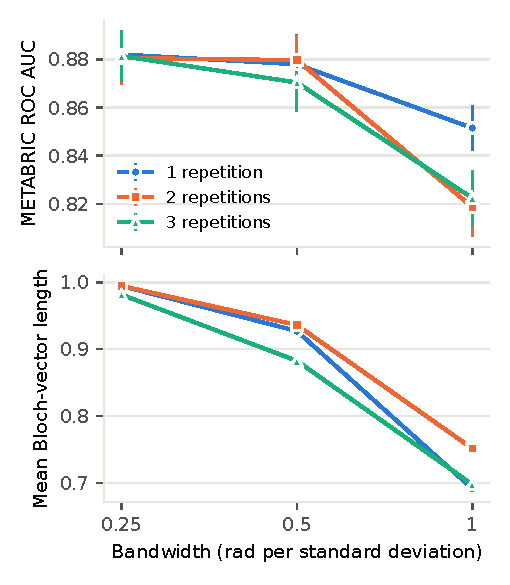
\includegraphics[width=\columnwidth]{figures/bandwidth.pdf}
\caption{\label{fig:bandwidth}METABRIC ROC AUC (top) and mean Bloch-vector length (bottom) against the bandwidth $\beta$, averaged over sizes. Bars are one standard error over resamples.}
\end{figure}

\subsection{Concentration}

At fixed depth and bandwidth, the mean Bloch-vector length varies by at most \ConcBloch{} and the spread of the features by at most \ConcSpread{} as the number of qubits goes from 20 to 156.
This follows from locality: each feature depends only on its light cone, whose size is bounded at fixed $R$ (Table~\ref{tab:cones}).
The relative spread of pairwise distances decreases slowly with $n$ for the PQK features and for the raw classical features alike.
% Numbers: results/scaling.csv, columns bloch_norm, feature_spread, d2_cv; notebook 3, Sec. 3.6.

\subsection{Entanglement ablation}
\label{sec:ablation}

Table~\ref{tab:ablation} adds two controls.
The first removes every two-qubit gate from the feature map, which leaves a product state.
The second gives the RBF-SVM inputs clipped at three standard deviations, as the circuit receives them.
Under cohort-wise standardization all five models agree within their standard errors.
Under per-sample rank normalization the kernel models are less stable.
In one of the five resamples the plain RBF-SVM loses more than 0.1 in METABRIC AUC at 100 and at 156 qubits, and the PQK does so at 100 qubits.
The two controls and logistic regression are affected less.
In every column the PQK and its entangler-free version agree within one standard error.

\begin{table}
\caption{\label{tab:ablation}ROC AUC on METABRIC under two normalizations. Mean over 5 resamples, standard error in parentheses.}
\resizebox{\columnwidth}{!}{\begin{tabular}{lccc}
\toprule
Model & $n=20$ & $n=100$ & $n=156$ \\
\midrule
\multicolumn{4}{l}{\textit{Cohort-wise $z$-score}} \\
PQK & 0.884(10) & 0.880(8) & 0.886(9) \\
PQK, entanglers removed & 0.882(9) & 0.880(8) & 0.881(10) \\
RBF-SVM & 0.873(17) & 0.883(4) & 0.881(8) \\
RBF-SVM, clipped inputs & 0.881(10) & 0.884(4) & 0.883(8) \\
Logistic regression & 0.880(10) & 0.875(10) & 0.879(6) \\
\addlinespace
\multicolumn{4}{l}{\textit{Per-sample rank}} \\
PQK & 0.877(5) & 0.848(36) & 0.876(8) \\
PQK, entanglers removed & 0.877(5) & 0.868(20) & 0.871(14) \\
RBF-SVM & 0.876(6) & 0.850(39) & 0.860(24) \\
RBF-SVM, clipped inputs & 0.876(5) & 0.870(17) & 0.875(12) \\
Logistic regression & 0.873(6) & 0.877(7) & 0.874(11) \\
\bottomrule
\end{tabular}
}
\end{table}

\subsection{Classical simulability}

Every result in this draft was obtained classically (Sec.~\ref{sec:sim}).
At the depths that cross-validation selects, the largest light cone holds at most 13 qubits.
Cones beyond direct statevector simulation require $R\ge 5$ (Table~\ref{tab:cones}).

\subsection{Shot budget and hardware cost}

No hardware runs are included in this draft. This subsection records the planning numbers.

Table~\ref{tab:proxy} shows a first-order noise proxy at the selected feature maps.
Each expectation value is multiplied by $(1-\epsilon)^{m_k}$, where $m_k$ is the number of CZ gates in the light cone of qubit $k$ and $\epsilon=\ProxyEps$ is the median CZ error of the calibration snapshot,
and is then sampled with a finite number of shots per basis.
The proxy ignores crosstalk, leakage, and readout bias.

\begin{table}
\caption{\label{tab:proxy}Noise proxy: ROC AUC on METABRIC at the selected feature maps, against the number of shots per measurement basis. Mean over \NSeeds{} resamples.}
\begin{tabular}{rcccc}
\toprule
Qubits & Exact & 4096 shots & 1024 shots & 256 shots \\
\midrule
20 & 0.884 & 0.884 & 0.875 & 0.882 \\
40 & 0.881 & 0.889 & 0.885 & 0.880 \\
60 & 0.869 & 0.865 & 0.866 & 0.859 \\
80 & 0.875 & 0.877 & 0.872 & 0.890 \\
100 & 0.882 & 0.878 & 0.879 & 0.882 \\
127 & 0.866 & 0.865 & 0.876 & 0.872 \\
156 & 0.888 & 0.883 & 0.887 & 0.888 \\
\bottomrule
\end{tabular}

\end{table}

The circuits are short. At $R=2$ on 156 qubits the transpiled circuit lasts \CircuitUs~$\mu$s, against a default repetition delay of \RepDelayUs~$\mu$s.
The cost is therefore set by the number of samples and shots, not by the number of qubits or the depth.
With three measurement bases, 600 tumors at 1024 shots take an estimated \MinFull~min of processor time per configuration, and \MinFullHigh~min at 4096 shots.
These estimates include a factor 1.5 for overhead, which is a guess to be replaced by the billed time of a pilot run.
The planned runs use readout mitigation only~\cite{trex}, with the feature map transpiled once and all tumors supplied as parameter values.

% ---------------------------------------------------------------------------
% \section{Hardware results}      TO ADD after the runs on ibm_fez (notebook 4).
% \section{Discussion}            TO WRITE.
% Points to cover: bandwidth and concentration~\cite{thanasilp2024,shaydulin2022,canatar2023};
% the shallow circuits that classify well are the ones that are classically simulable.
% ---------------------------------------------------------------------------

\FloatBarrier

\begin{thebibliography}{99}

\bibitem{tcga2012} The Cancer Genome Atlas Network, Comprehensive molecular portraits of human breast tumours, Nature \textbf{490}, 61 (2012).

\bibitem{ciriello2015} G. Ciriello \textit{et al.}, Comprehensive molecular portraits of invasive lobular breast cancer, Cell \textbf{163}, 506 (2015).

\bibitem{hoadley2018} K. A. Hoadley \textit{et al.}, Cell-of-origin patterns dominate the molecular classification of 10,000 tumors from 33 types of cancer, Cell \textbf{173}, 291 (2018).

\bibitem{curtis2012} C. Curtis \textit{et al.}, The genomic and transcriptomic architecture of 2,000 breast tumours reveals novel subgroups, Nature \textbf{486}, 346 (2012).

\bibitem{pereira2016} B. Pereira \textit{et al.}, The somatic mutation profiles of 2,433 breast cancers refines their genomic and transcriptomic landscapes, Nat. Commun. \textbf{7}, 11479 (2016).

\bibitem{cerami2012} E. Cerami \textit{et al.}, The cBio Cancer Genomics Portal: an open platform for exploring multidimensional cancer genomics data, Cancer Discov. \textbf{2}, 401 (2012).

\bibitem{gao2013} J. Gao \textit{et al.}, Integrative analysis of complex cancer genomics and clinical profiles using the cBioPortal, Sci. Signal. \textbf{6}, pl1 (2013).

\bibitem{huang2021} H.-Y. Huang, M. Broughton, M. Mohseni, R. Babbush, S. Boixo, H. Neven, and J. R. McClean, Power of data in quantum machine learning, Nat. Commun. \textbf{12}, 2631 (2021).

\bibitem{sklearn} F. Pedregosa \textit{et al.}, Scikit-learn: machine learning in Python, J. Mach. Learn. Res. \textbf{12}, 2825 (2011).

\bibitem{qiskit} A. Javadi-Abhari \textit{et al.}, Quantum computing with Qiskit, arXiv:2405.08810 (2024).

\bibitem{trex} E. van den Berg, Z. K. Minev, and K. Temme, Model-free readout-error mitigation for quantum expectation values, Phys. Rev. A \textbf{105}, 032620 (2022).

% For the discussion:
% \bibitem{thanasilp2024} S. Thanasilp, S. Wang, M. Cerezo, and Z. Holmes, Exponential concentration in quantum kernel methods, Nat. Commun. \textbf{15}, 5200 (2024).
% \bibitem{shaydulin2022} R. Shaydulin and S. M. Wild, Importance of kernel bandwidth in quantum machine learning, Phys. Rev. A \textbf{106}, 042407 (2022).
% \bibitem{canatar2023} A. Canatar, E. Peters, C. Pehlevan, S. M. Wild, and R. Shaydulin, Bandwidth enables generalization in quantum kernel models, Trans. Mach. Learn. Res. (2023).

\end{thebibliography}

\end{document}
